% Options for packages loaded elsewhere
\PassOptionsToPackage{unicode}{hyperref}
\PassOptionsToPackage{hyphens}{url}
%
\documentclass[
]{article}
\usepackage{amsmath,amssymb}
\usepackage{iftex}
\ifPDFTeX
  \usepackage[T1]{fontenc}
  \usepackage[utf8]{inputenc}
  \usepackage{textcomp} % provide euro and other symbols
\else % if luatex or xetex
  \usepackage{unicode-math} % this also loads fontspec
  \defaultfontfeatures{Scale=MatchLowercase}
  \defaultfontfeatures[\rmfamily]{Ligatures=TeX,Scale=1}
\fi
\usepackage{lmodern}
\ifPDFTeX\else
  % xetex/luatex font selection
\fi
% Use upquote if available, for straight quotes in verbatim environments
\IfFileExists{upquote.sty}{\usepackage{upquote}}{}
\IfFileExists{microtype.sty}{% use microtype if available
  \usepackage[]{microtype}
  \UseMicrotypeSet[protrusion]{basicmath} % disable protrusion for tt fonts
}{}
\makeatletter
\@ifundefined{KOMAClassName}{% if non-KOMA class
  \IfFileExists{parskip.sty}{%
    \usepackage{parskip}
  }{% else
    \setlength{\parindent}{0pt}
    \setlength{\parskip}{6pt plus 2pt minus 1pt}}
}{% if KOMA class
  \KOMAoptions{parskip=half}}
\makeatother
\usepackage{xcolor}
\usepackage[margin=1in]{geometry}
\usepackage{color}
\usepackage{fancyvrb}
\newcommand{\VerbBar}{|}
\newcommand{\VERB}{\Verb[commandchars=\\\{\}]}
\DefineVerbatimEnvironment{Highlighting}{Verbatim}{commandchars=\\\{\}}
% Add ',fontsize=\small' for more characters per line
\usepackage{framed}
\definecolor{shadecolor}{RGB}{248,248,248}
\newenvironment{Shaded}{\begin{snugshade}}{\end{snugshade}}
\newcommand{\AlertTok}[1]{\textcolor[rgb]{0.94,0.16,0.16}{#1}}
\newcommand{\AnnotationTok}[1]{\textcolor[rgb]{0.56,0.35,0.01}{\textbf{\textit{#1}}}}
\newcommand{\AttributeTok}[1]{\textcolor[rgb]{0.13,0.29,0.53}{#1}}
\newcommand{\BaseNTok}[1]{\textcolor[rgb]{0.00,0.00,0.81}{#1}}
\newcommand{\BuiltInTok}[1]{#1}
\newcommand{\CharTok}[1]{\textcolor[rgb]{0.31,0.60,0.02}{#1}}
\newcommand{\CommentTok}[1]{\textcolor[rgb]{0.56,0.35,0.01}{\textit{#1}}}
\newcommand{\CommentVarTok}[1]{\textcolor[rgb]{0.56,0.35,0.01}{\textbf{\textit{#1}}}}
\newcommand{\ConstantTok}[1]{\textcolor[rgb]{0.56,0.35,0.01}{#1}}
\newcommand{\ControlFlowTok}[1]{\textcolor[rgb]{0.13,0.29,0.53}{\textbf{#1}}}
\newcommand{\DataTypeTok}[1]{\textcolor[rgb]{0.13,0.29,0.53}{#1}}
\newcommand{\DecValTok}[1]{\textcolor[rgb]{0.00,0.00,0.81}{#1}}
\newcommand{\DocumentationTok}[1]{\textcolor[rgb]{0.56,0.35,0.01}{\textbf{\textit{#1}}}}
\newcommand{\ErrorTok}[1]{\textcolor[rgb]{0.64,0.00,0.00}{\textbf{#1}}}
\newcommand{\ExtensionTok}[1]{#1}
\newcommand{\FloatTok}[1]{\textcolor[rgb]{0.00,0.00,0.81}{#1}}
\newcommand{\FunctionTok}[1]{\textcolor[rgb]{0.13,0.29,0.53}{\textbf{#1}}}
\newcommand{\ImportTok}[1]{#1}
\newcommand{\InformationTok}[1]{\textcolor[rgb]{0.56,0.35,0.01}{\textbf{\textit{#1}}}}
\newcommand{\KeywordTok}[1]{\textcolor[rgb]{0.13,0.29,0.53}{\textbf{#1}}}
\newcommand{\NormalTok}[1]{#1}
\newcommand{\OperatorTok}[1]{\textcolor[rgb]{0.81,0.36,0.00}{\textbf{#1}}}
\newcommand{\OtherTok}[1]{\textcolor[rgb]{0.56,0.35,0.01}{#1}}
\newcommand{\PreprocessorTok}[1]{\textcolor[rgb]{0.56,0.35,0.01}{\textit{#1}}}
\newcommand{\RegionMarkerTok}[1]{#1}
\newcommand{\SpecialCharTok}[1]{\textcolor[rgb]{0.81,0.36,0.00}{\textbf{#1}}}
\newcommand{\SpecialStringTok}[1]{\textcolor[rgb]{0.31,0.60,0.02}{#1}}
\newcommand{\StringTok}[1]{\textcolor[rgb]{0.31,0.60,0.02}{#1}}
\newcommand{\VariableTok}[1]{\textcolor[rgb]{0.00,0.00,0.00}{#1}}
\newcommand{\VerbatimStringTok}[1]{\textcolor[rgb]{0.31,0.60,0.02}{#1}}
\newcommand{\WarningTok}[1]{\textcolor[rgb]{0.56,0.35,0.01}{\textbf{\textit{#1}}}}
\usepackage{graphicx}
\makeatletter
\def\maxwidth{\ifdim\Gin@nat@width>\linewidth\linewidth\else\Gin@nat@width\fi}
\def\maxheight{\ifdim\Gin@nat@height>\textheight\textheight\else\Gin@nat@height\fi}
\makeatother
% Scale images if necessary, so that they will not overflow the page
% margins by default, and it is still possible to overwrite the defaults
% using explicit options in \includegraphics[width, height, ...]{}
\setkeys{Gin}{width=\maxwidth,height=\maxheight,keepaspectratio}
% Set default figure placement to htbp
\makeatletter
\def\fps@figure{htbp}
\makeatother
\setlength{\emergencystretch}{3em} % prevent overfull lines
\providecommand{\tightlist}{%
  \setlength{\itemsep}{0pt}\setlength{\parskip}{0pt}}
\setcounter{secnumdepth}{-\maxdimen} % remove section numbering
\ifLuaTeX
  \usepackage{selnolig}  % disable illegal ligatures
\fi
\IfFileExists{bookmark.sty}{\usepackage{bookmark}}{\usepackage{hyperref}}
\IfFileExists{xurl.sty}{\usepackage{xurl}}{} % add URL line breaks if available
\urlstyle{same}
\hypersetup{
  hidelinks,
  pdfcreator={LaTeX via pandoc}}

\author{}
\date{\vspace{-2.5em}}

\begin{document}

In this example, we perform tuning of an MLP using \texttt{nnet} and
\texttt{neuralnet} for a classification problem.

Although the neuralnet package can deal directly with classification
problems, including factor-valued variables, this is not possible within
the caret framework and we have to perform a one-hot encoding on the
data in a preprocessing step. This encoding converts class values to
numerical values, equal to either zero or one. In the case of the iris
data, where there are 3 possible levels of the \texttt{Species}
factor---the response variable---we need to add 3 columns, one
corresponding to each level/species, whose values will be either 1 or 0
depending on whether the given observation belongs to a given species,
or not. Then the classification problem can be treated as a regression
problem by caret's \texttt{neuralnet} method.

We use the Iris Data Set downloaded from the kaggle site
{[}{]}{[}\url{https://www.kaggle.com/uciml/iris}{]}.

Step1: Read in the required packages and data.

\begin{Shaded}
\begin{Highlighting}[]
\CommentTok{\#Load required packages}
\FunctionTok{library}\NormalTok{(neuralnet)}
\FunctionTok{library}\NormalTok{(caret)}
\FunctionTok{library}\NormalTok{(reshape2)}
\FunctionTok{library}\NormalTok{(ggplot2)}
\FunctionTok{library}\NormalTok{(stringr)}
\CommentTok{\#Read  data}
\NormalTok{irisData }\OtherTok{\textless{}{-}} \FunctionTok{read.csv}\NormalTok{(}\AttributeTok{file=}\StringTok{"iris.csv"}\NormalTok{, }\AttributeTok{head =} \ConstantTok{TRUE}\NormalTok{, }\AttributeTok{sep =} \StringTok{","}\NormalTok{)}
\end{Highlighting}
\end{Shaded}

Step 2: (EDA) Inspect the data.

\begin{Shaded}
\begin{Highlighting}[]
\CommentTok{\#Get a summary of the data}
\FunctionTok{summary}\NormalTok{(irisData)}
\end{Highlighting}
\end{Shaded}

\begin{verbatim}
##        Id         SepalLengthCm    SepalWidthCm   PetalLengthCm  
##  Min.   :  1.00   Min.   :4.300   Min.   :2.000   Min.   :1.000  
##  1st Qu.: 38.25   1st Qu.:5.100   1st Qu.:2.800   1st Qu.:1.600  
##  Median : 75.50   Median :5.800   Median :3.000   Median :4.350  
##  Mean   : 75.50   Mean   :5.843   Mean   :3.054   Mean   :3.759  
##  3rd Qu.:112.75   3rd Qu.:6.400   3rd Qu.:3.300   3rd Qu.:5.100  
##  Max.   :150.00   Max.   :7.900   Max.   :4.400   Max.   :6.900  
##   PetalWidthCm     Species         
##  Min.   :0.100   Length:150        
##  1st Qu.:0.300   Class :character  
##  Median :1.300   Mode  :character  
##  Mean   :1.199                     
##  3rd Qu.:1.800                     
##  Max.   :2.500
\end{verbatim}

\begin{Shaded}
\begin{Highlighting}[]
\FunctionTok{str}\NormalTok{(irisData)}
\end{Highlighting}
\end{Shaded}

\begin{verbatim}
## 'data.frame':    150 obs. of  6 variables:
##  $ Id           : int  1 2 3 4 5 6 7 8 9 10 ...
##  $ SepalLengthCm: num  5.1 4.9 4.7 4.6 5 5.4 4.6 5 4.4 4.9 ...
##  $ SepalWidthCm : num  3.5 3 3.2 3.1 3.6 3.9 3.4 3.4 2.9 3.1 ...
##  $ PetalLengthCm: num  1.4 1.4 1.3 1.5 1.4 1.7 1.4 1.5 1.4 1.5 ...
##  $ PetalWidthCm : num  0.2 0.2 0.2 0.2 0.2 0.4 0.3 0.2 0.2 0.1 ...
##  $ Species      : chr  "Iris-setosa" "Iris-setosa" "Iris-setosa" "Iris-setosa" ...
\end{verbatim}

Step 3: (EDA) Check the data for any missing values. There are multiple
ways to do this but. Here, we use the \texttt{colsums} function to
determine how many missing values are in each column, if any.

\begin{Shaded}
\begin{Highlighting}[]
\CommentTok{\#Compute total number of NA values in each column. Note, this  will be tricked if there are dummy values standing in for true missing data. }
\FunctionTok{colSums}\NormalTok{(}\FunctionTok{is.na}\NormalTok{(irisData))}
\end{Highlighting}
\end{Shaded}

\begin{verbatim}
##            Id SepalLengthCm  SepalWidthCm PetalLengthCm  PetalWidthCm 
##             0             0             0             0             0 
##       Species 
##             0
\end{verbatim}

Step 4: Perform any required data cleaning. Here, we remove the
``Iris-'' from the species column. Otherwise, if left in, could cause
difficulties in constructing the model formula automatically.

\begin{Shaded}
\begin{Highlighting}[]
\NormalTok{irisData}\SpecialCharTok{$}\NormalTok{Species }\OtherTok{\textless{}{-}} \FunctionTok{str\_replace}\NormalTok{(irisData}\SpecialCharTok{$}\NormalTok{Species, }\StringTok{"Iris{-}"}\NormalTok{,}\StringTok{""}\NormalTok{)}
\end{Highlighting}
\end{Shaded}

Step 5: Look at the data graphically, to choose the best predictors for
a model.

\begin{Shaded}
\begin{Highlighting}[]
\FunctionTok{ggplot}\NormalTok{(irisData, }\FunctionTok{aes}\NormalTok{(SepalLengthCm, SepalWidthCm, }\AttributeTok{color =}\NormalTok{ Species)) }\SpecialCharTok{+} \FunctionTok{geom\_point}\NormalTok{()}
\end{Highlighting}
\end{Shaded}

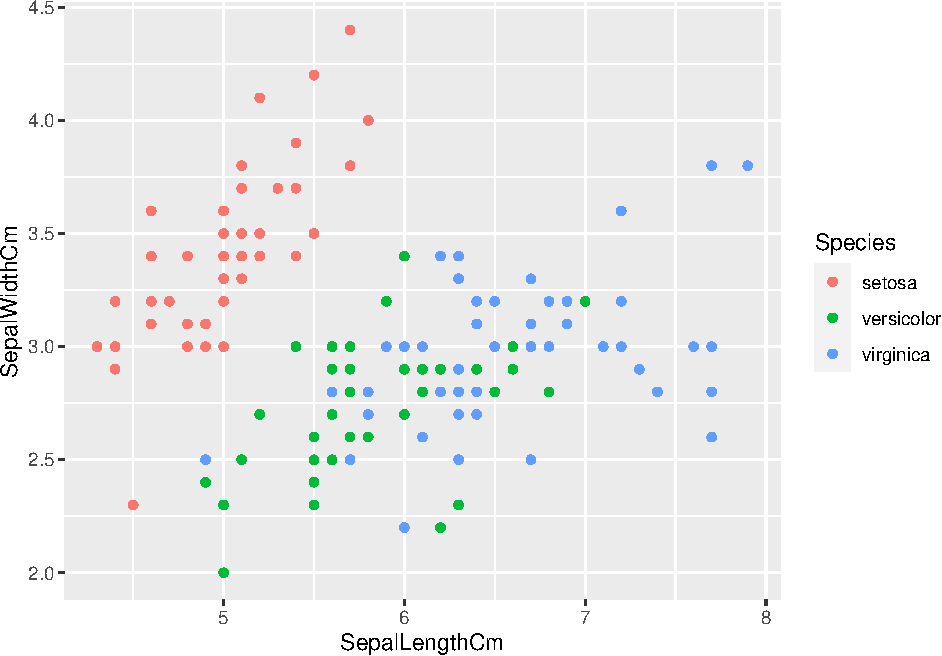
\includegraphics{nn_class_caret_tune_files/figure-latex/unnamed-chunk-5-1.pdf}

\begin{Shaded}
\begin{Highlighting}[]
\FunctionTok{ggplot}\NormalTok{(irisData, }\FunctionTok{aes}\NormalTok{(PetalLengthCm, PetalWidthCm, }\AttributeTok{color =}\NormalTok{ Species)) }\SpecialCharTok{+} \FunctionTok{geom\_point}\NormalTok{()}
\end{Highlighting}
\end{Shaded}

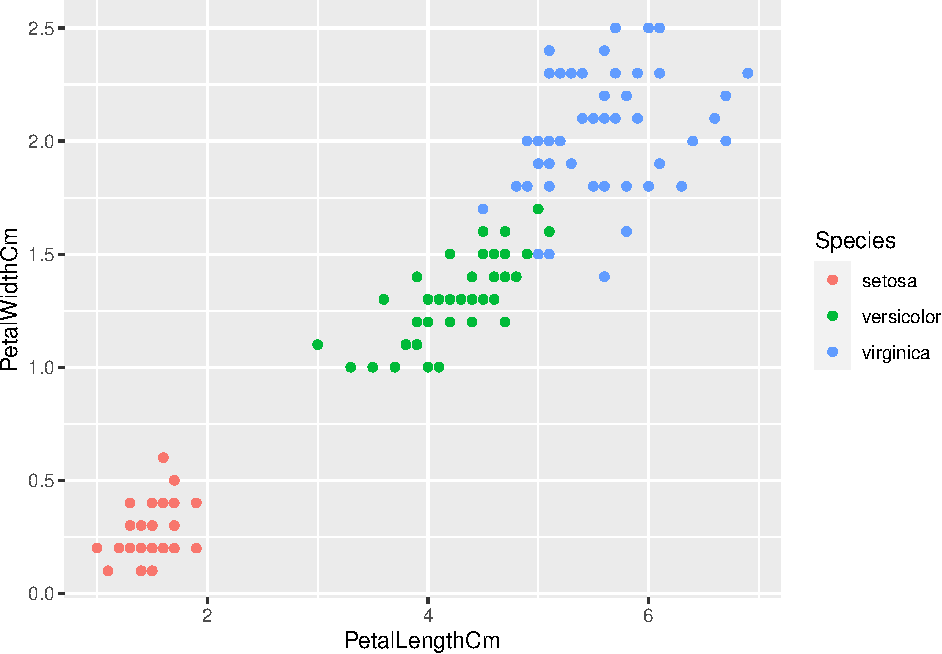
\includegraphics{nn_class_caret_tune_files/figure-latex/unnamed-chunk-5-2.pdf}

Step 6: To use the measurements in the neural network, it is
indispensable to normalize or scale them. If it is not scaled, the model
will either be difficult to train---will not converge---or will result
in uninterpretable results. We only scale the feature columns.

\begin{Shaded}
\begin{Highlighting}[]
\NormalTok{irisData[,}\DecValTok{2}\SpecialCharTok{:}\DecValTok{5}\NormalTok{] }\OtherTok{\textless{}{-}} \FunctionTok{scale}\NormalTok{(irisData[,}\DecValTok{2}\SpecialCharTok{:}\DecValTok{5}\NormalTok{])}
\end{Highlighting}
\end{Shaded}

Step 7: Because the \texttt{neuralnet} method within \texttt{caret} does
not accept factors, the outcome variable needs to be adjusted. We use
the \texttt{cbind} command to perform one-hot encoding, thus adding 3
columns with transformations of the outcome variable into target
vectors.

\begin{Shaded}
\begin{Highlighting}[]
\NormalTok{irisData }\OtherTok{\textless{}{-}} \FunctionTok{cbind}\NormalTok{(irisData, }\FunctionTok{model.matrix}\NormalTok{(}\SpecialCharTok{\textasciitilde{}} \DecValTok{0} \SpecialCharTok{+}\NormalTok{ Species, irisData))}
\CommentTok{\# check the one{-}hot encoding}
\FunctionTok{head}\NormalTok{(irisData[,}\DecValTok{6}\SpecialCharTok{:}\DecValTok{9}\NormalTok{])}
\end{Highlighting}
\end{Shaded}

\begin{verbatim}
##   Species Speciessetosa Speciesversicolor Speciesvirginica
## 1  setosa             1                 0                0
## 2  setosa             1                 0                0
## 3  setosa             1                 0                0
## 4  setosa             1                 0                0
## 5  setosa             1                 0                0
## 6  setosa             1                 0                0
\end{verbatim}

\begin{Shaded}
\begin{Highlighting}[]
\FunctionTok{tail}\NormalTok{(irisData[,}\DecValTok{6}\SpecialCharTok{:}\DecValTok{9}\NormalTok{])}
\end{Highlighting}
\end{Shaded}

\begin{verbatim}
##       Species Speciessetosa Speciesversicolor Speciesvirginica
## 145 virginica             0                 0                1
## 146 virginica             0                 0                1
## 147 virginica             0                 0                1
## 148 virginica             0                 0                1
## 149 virginica             0                 0                1
## 150 virginica             0                 0                1
\end{verbatim}

Step 8: Split the data into training and testing data in the proportion
75\% for training and 25\% for testing.

\begin{Shaded}
\begin{Highlighting}[]
\CommentTok{\#set the seed to get reproducible results}
\FunctionTok{set.seed}\NormalTok{(}\DecValTok{12345}\NormalTok{)}
\NormalTok{inTrain }\OtherTok{\textless{}{-}} \FunctionTok{createDataPartition}\NormalTok{(}\AttributeTok{y=}\NormalTok{irisData}\SpecialCharTok{$}\NormalTok{Species, }\AttributeTok{p=}\FloatTok{0.75}\NormalTok{, }\AttributeTok{list=}\ConstantTok{FALSE}\NormalTok{)}
\NormalTok{train.set }\OtherTok{\textless{}{-}}\NormalTok{ irisData[inTrain,]}
\NormalTok{test.set  }\OtherTok{\textless{}{-}}\NormalTok{ irisData[}\SpecialCharTok{{-}}\NormalTok{inTrain,]}
\end{Highlighting}
\end{Shaded}

Step 9: Create the model formula.

\begin{Shaded}
\begin{Highlighting}[]
\CommentTok{\#Get the variable names for the input and output}
\NormalTok{predictorVars }\OtherTok{\textless{}{-}} \FunctionTok{names}\NormalTok{(irisData)[}\DecValTok{2}\SpecialCharTok{:}\DecValTok{5}\NormalTok{]}
\NormalTok{outcomeVars   }\OtherTok{\textless{}{-}} \FunctionTok{names}\NormalTok{(irisData)[}\DecValTok{7}\SpecialCharTok{:}\DecValTok{9}\NormalTok{]}
\CommentTok{\#Paste together the formula }
\NormalTok{modFormula }\OtherTok{\textless{}{-}} \FunctionTok{as.formula}\NormalTok{(}\FunctionTok{paste}\NormalTok{(}\FunctionTok{paste}\NormalTok{(outcomeVars, }\AttributeTok{collapse =} \StringTok{"+"}\NormalTok{),}
                               \StringTok{"\textasciitilde{}"}\NormalTok{, }\FunctionTok{paste}\NormalTok{(predictorVars, }\AttributeTok{collapse =} \StringTok{" + "}\NormalTok{)))}
\NormalTok{modFormula}
\end{Highlighting}
\end{Shaded}

\begin{verbatim}
## Speciessetosa + Speciesversicolor + Speciesvirginica ~ SepalLengthCm + 
##     SepalWidthCm + PetalLengthCm + PetalWidthCm
\end{verbatim}

Step 10: Train the network. There are no fixed rules for the
hyperparameters, threshold, steps and hidden layers. These can be tuned
in order to improve the network performance.

\begin{Shaded}
\begin{Highlighting}[]
\NormalTok{irisNNet }\OtherTok{\textless{}{-}} \FunctionTok{neuralnet}\NormalTok{(}\AttributeTok{formula =}\NormalTok{ modFormula, }
                     \AttributeTok{data =}\NormalTok{ train.set, }
                     \AttributeTok{hidden =} \FunctionTok{c}\NormalTok{(}\DecValTok{4}\NormalTok{), }
                     \AttributeTok{linear.output =} \ConstantTok{FALSE}\NormalTok{, }
                     \AttributeTok{threshold =}\NormalTok{ .}\DecValTok{05}\NormalTok{, }
                     \AttributeTok{stepmax =} \DecValTok{5000}\NormalTok{)}
\end{Highlighting}
\end{Shaded}

Step 11: See how well the network did by computing its classification
accuracy.

\begin{Shaded}
\begin{Highlighting}[]
\NormalTok{classes }\OtherTok{\textless{}{-}} \FunctionTok{compute}\NormalTok{(irisNNet, test.set)}
\CommentTok{\#Get the classification results out of classes}
\NormalTok{classRes }\OtherTok{\textless{}{-}}\NormalTok{ classes}\SpecialCharTok{$}\NormalTok{net.result}
\CommentTok{\#Using the apply funciton in conjunction with the \textquotesingle{}which.max\textquotesingle{} function to get the max index }
\CommentTok{\#for each row of the classRes matrix and the test rows of original data}
\NormalTok{nnClass }\OtherTok{\textless{}{-}} \FunctionTok{apply}\NormalTok{(classRes, }\AttributeTok{MARGIN =} \DecValTok{1}\NormalTok{, which.max)}
\NormalTok{origClass }\OtherTok{\textless{}{-}} \FunctionTok{apply}\NormalTok{(test.set[, }\FunctionTok{c}\NormalTok{(}\DecValTok{7}\SpecialCharTok{:}\DecValTok{9}\NormalTok{)], }\AttributeTok{MARGIN =} \DecValTok{1}\NormalTok{, which.max)  }
\CommentTok{\#Compute the percentage of correct classification for the neural network: }
\CommentTok{\# \textquotesingle{}round\textquotesingle{} is testing pr \textgreater{} 0.5 ?}
\CommentTok{\# \textquotesingle{}mean\textquotesingle{} gives the probability of each class}
\CommentTok{\# \textquotesingle{}100\textquotesingle{} gives the percentage}
\FunctionTok{paste}\NormalTok{(}\StringTok{"The classification accuracy of the network is"}\NormalTok{, }
      \FunctionTok{round}\NormalTok{(}\FunctionTok{mean}\NormalTok{(nnClass }\SpecialCharTok{==}\NormalTok{ origClass) }\SpecialCharTok{*} \DecValTok{100}\NormalTok{, }\AttributeTok{digits =} \DecValTok{2}\NormalTok{), }\StringTok{"\%"}\NormalTok{)}
\end{Highlighting}
\end{Shaded}

\begin{verbatim}
## [1] "The classification accuracy of the network is 97.22 %"
\end{verbatim}

Although these seem like good results this may simply be a result of the
partition into training and testing data, so it is important to test the
model performance further. Here, we manually perform k-fold cross
validation using 10 folds (10 fold cross-validation).

Step 12: Validate the Model

\begin{Shaded}
\begin{Highlighting}[]
\CommentTok{\#Compute the testing indices using the createFolds function of caret}
\NormalTok{folds }\OtherTok{\textless{}{-}} \FunctionTok{createFolds}\NormalTok{(irisData}\SpecialCharTok{$}\NormalTok{Species, }\AttributeTok{k =} \DecValTok{10}\NormalTok{)}
\CommentTok{\#\textquotesingle{}results\textquotesingle{} is a vector that will contain the accuracy for each fold}
\CommentTok{\# of the network training and testing}
\NormalTok{results }\OtherTok{\textless{}{-}} \FunctionTok{c}\NormalTok{()}
\ControlFlowTok{for}\NormalTok{ (fld }\ControlFlowTok{in}\NormalTok{ folds)\{}
  \CommentTok{\# train the network }
\NormalTok{  nn }\OtherTok{\textless{}{-}} \FunctionTok{neuralnet}\NormalTok{(}\AttributeTok{formula =}\NormalTok{ modFormula, }\AttributeTok{data =}\NormalTok{ irisData[}\SpecialCharTok{{-}}\NormalTok{fld,], }\AttributeTok{hidden =} \FunctionTok{c}\NormalTok{(}\DecValTok{4}\NormalTok{), }
                  \AttributeTok{linear.output =} \ConstantTok{FALSE}\NormalTok{, }\AttributeTok{threshold =}\NormalTok{ .}\DecValTok{05}\NormalTok{, }\AttributeTok{stepmax =} \DecValTok{5000}\NormalTok{)}
  \CommentTok{\# extract the classifications from the network}
\NormalTok{  classes }\OtherTok{\textless{}{-}} \FunctionTok{compute}\NormalTok{(nn, irisData[fld ,}\SpecialCharTok{{-}}\FunctionTok{c}\NormalTok{(}\DecValTok{1}\NormalTok{,}\DecValTok{6}\SpecialCharTok{:}\DecValTok{9}\NormalTok{)])}
  \CommentTok{\# check the accuracy of the network using the same procedure as above}
\NormalTok{  classRes }\OtherTok{\textless{}{-}}\NormalTok{ classes}\SpecialCharTok{$}\NormalTok{net.result}
\NormalTok{  nnClass }\OtherTok{\textless{}{-}} \FunctionTok{apply}\NormalTok{(classRes, }\AttributeTok{MARGIN =} \DecValTok{1}\NormalTok{, which.max)}
\NormalTok{  origClass }\OtherTok{\textless{}{-}} \FunctionTok{apply}\NormalTok{(irisData[fld , }\FunctionTok{c}\NormalTok{(}\DecValTok{7}\SpecialCharTok{:}\DecValTok{9}\NormalTok{)], }\AttributeTok{MARGIN =} \DecValTok{1}\NormalTok{, which.max)  }
\NormalTok{  results }\OtherTok{\textless{}{-}} \FunctionTok{c}\NormalTok{(results, }\FunctionTok{mean}\NormalTok{(nnClass }\SpecialCharTok{==}\NormalTok{ origClass) }\SpecialCharTok{*} \DecValTok{100}\NormalTok{)}
\NormalTok{\} }
\CommentTok{\# outoput the result}
\FunctionTok{paste}\NormalTok{(}\StringTok{"After"}\NormalTok{, }\FunctionTok{length}\NormalTok{(results), }
      \StringTok{"validation loops the mean accuracy of the network is"}\NormalTok{, }
      \FunctionTok{paste0}\NormalTok{(}\FunctionTok{round}\NormalTok{(}\FunctionTok{mean}\NormalTok{(results),}\DecValTok{2}\NormalTok{), }\StringTok{"\%"}\NormalTok{))}
\end{Highlighting}
\end{Shaded}

\begin{verbatim}
## [1] "After 10 validation loops the mean accuracy of the network is 96%"
\end{verbatim}

Now, perform CV using the \texttt{caret} package.

\begin{Shaded}
\begin{Highlighting}[]
\CommentTok{\# Define the tuning grid}
\NormalTok{grid }\OtherTok{\textless{}{-}}  \FunctionTok{expand.grid}\NormalTok{(}\AttributeTok{size=}\FunctionTok{c}\NormalTok{(}\DecValTok{2}\NormalTok{,}\DecValTok{4}\NormalTok{), }\AttributeTok{decay=}\DecValTok{2}\SpecialCharTok{\^{}}\NormalTok{(}\SpecialCharTok{{-}}\DecValTok{3}\SpecialCharTok{:{-}}\DecValTok{1}\NormalTok{))}
\CommentTok{\# define the CV strategy}
\NormalTok{tr.nnet }\OtherTok{\textless{}{-}} \FunctionTok{trainControl}\NormalTok{(}\AttributeTok{method =} \StringTok{"cv"}\NormalTok{,}
                        \AttributeTok{number =} \DecValTok{5}\NormalTok{,}
                        \AttributeTok{verboseIter =} \ConstantTok{TRUE}\NormalTok{)}
\CommentTok{\# Train with \textasciigrave{}caret\textasciigrave{} }
\NormalTok{nn1 }\OtherTok{\textless{}{-}} \FunctionTok{train}\NormalTok{(Species }\SpecialCharTok{\textasciitilde{}}\NormalTok{., }\CommentTok{\#formula = modFormula, }
            \AttributeTok{data =}\NormalTok{ train.set[,}\DecValTok{1}\SpecialCharTok{:}\DecValTok{6}\NormalTok{], }
            \AttributeTok{method=}\StringTok{"nnet"}\NormalTok{,}\CommentTok{\#method = "neuralnet", }
            \AttributeTok{tuneGrid =}\NormalTok{ grid,}
            \AttributeTok{preProc =} \FunctionTok{c}\NormalTok{(}\StringTok{"center"}\NormalTok{, }\StringTok{"scale"}\NormalTok{, }\StringTok{"nzv"}\NormalTok{), }
            \AttributeTok{trControl =}\NormalTok{ tr.nnet)}
\end{Highlighting}
\end{Shaded}

\begin{verbatim}
## + Fold1: size=2, decay=0.125 
## # weights:  21
## initial  value 111.704526 
## iter  10 value 22.888788
## iter  20 value 18.663312
## final  value 18.661892 
## converged
## - Fold1: size=2, decay=0.125 
## + Fold1: size=4, decay=0.125 
## # weights:  39
## initial  value 98.988268 
## iter  10 value 19.480327
## iter  20 value 17.078020
## iter  30 value 17.072665
## final  value 17.072665 
## converged
## - Fold1: size=4, decay=0.125 
## + Fold1: size=2, decay=0.250 
## # weights:  21
## initial  value 105.585293 
## iter  10 value 35.050588
## iter  20 value 29.152157
## iter  30 value 29.105871
## final  value 29.105871 
## converged
## - Fold1: size=2, decay=0.250 
## + Fold1: size=4, decay=0.250 
## # weights:  39
## initial  value 129.079239 
## iter  10 value 27.820488
## iter  20 value 24.089594
## iter  30 value 23.811317
## iter  40 value 23.810869
## iter  40 value 23.810869
## iter  40 value 23.810869
## final  value 23.810869 
## converged
## - Fold1: size=4, decay=0.250 
## + Fold1: size=2, decay=0.500 
## # weights:  21
## initial  value 110.784584 
## iter  10 value 48.150471
## iter  20 value 44.088273
## final  value 44.082612 
## converged
## - Fold1: size=2, decay=0.500 
## + Fold1: size=4, decay=0.500 
## # weights:  39
## initial  value 114.648922 
## iter  10 value 40.405027
## iter  20 value 37.760951
## iter  30 value 37.755432
## final  value 37.755416 
## converged
## - Fold1: size=4, decay=0.500 
## + Fold2: size=2, decay=0.125 
## # weights:  21
## initial  value 101.039006 
## iter  10 value 24.215441
## iter  20 value 18.680372
## iter  30 value 18.599284
## final  value 18.599114 
## converged
## - Fold2: size=2, decay=0.125 
## + Fold2: size=4, decay=0.125 
## # weights:  39
## initial  value 104.890567 
## iter  10 value 18.002740
## iter  20 value 14.957767
## iter  30 value 14.876416
## iter  40 value 14.876384
## final  value 14.876384 
## converged
## - Fold2: size=4, decay=0.125 
## + Fold2: size=2, decay=0.250 
## # weights:  21
## initial  value 104.384683 
## iter  10 value 37.346807
## iter  20 value 29.154016
## final  value 29.033976 
## converged
## - Fold2: size=2, decay=0.250 
## + Fold2: size=4, decay=0.250 
## # weights:  39
## initial  value 100.027669 
## iter  10 value 35.057910
## iter  20 value 24.348119
## iter  30 value 23.827182
## iter  40 value 23.825065
## final  value 23.825055 
## converged
## - Fold2: size=4, decay=0.250 
## + Fold2: size=2, decay=0.500 
## # weights:  21
## initial  value 104.032192 
## iter  10 value 47.285594
## iter  20 value 43.284413
## final  value 43.283151 
## converged
## - Fold2: size=2, decay=0.500 
## + Fold2: size=4, decay=0.500 
## # weights:  39
## initial  value 117.160549 
## iter  10 value 38.694214
## iter  20 value 36.632848
## iter  30 value 36.600448
## final  value 36.600434 
## converged
## - Fold2: size=4, decay=0.500 
## + Fold3: size=2, decay=0.125 
## # weights:  21
## initial  value 105.844547 
## iter  10 value 21.997533
## iter  20 value 18.428592
## final  value 18.421533 
## converged
## - Fold3: size=2, decay=0.125 
## + Fold3: size=4, decay=0.125 
## # weights:  39
## initial  value 104.304705 
## iter  10 value 21.587076
## iter  20 value 14.796379
## iter  30 value 14.396387
## iter  40 value 14.361763
## final  value 14.360886 
## converged
## - Fold3: size=4, decay=0.125 
## + Fold3: size=2, decay=0.250 
## # weights:  21
## initial  value 101.594902 
## iter  10 value 42.842600
## iter  20 value 28.488282
## iter  30 value 28.466019
## final  value 28.465965 
## converged
## - Fold3: size=2, decay=0.250 
## + Fold3: size=4, decay=0.250 
## # weights:  39
## initial  value 101.645135 
## iter  10 value 25.947652
## iter  20 value 23.199019
## iter  30 value 23.140566
## final  value 23.140435 
## converged
## - Fold3: size=4, decay=0.250 
## + Fold3: size=2, decay=0.500 
## # weights:  21
## initial  value 102.870560 
## iter  10 value 54.361393
## iter  20 value 42.701354
## final  value 42.695284 
## converged
## - Fold3: size=2, decay=0.500 
## + Fold3: size=4, decay=0.500 
## # weights:  39
## initial  value 108.580974 
## iter  10 value 39.889151
## iter  20 value 37.255652
## iter  30 value 37.150848
## final  value 37.150837 
## converged
## - Fold3: size=4, decay=0.500 
## + Fold4: size=2, decay=0.125 
## # weights:  21
## initial  value 110.299877 
## iter  10 value 20.140186
## iter  20 value 18.689777
## iter  30 value 18.682193
## final  value 18.682190 
## converged
## - Fold4: size=2, decay=0.125 
## + Fold4: size=4, decay=0.125 
## # weights:  39
## initial  value 106.396875 
## iter  10 value 17.297860
## iter  20 value 15.918761
## iter  30 value 15.906395
## final  value 15.905483 
## converged
## - Fold4: size=4, decay=0.125 
## + Fold4: size=2, decay=0.250 
## # weights:  21
## initial  value 109.165417 
## iter  10 value 34.378097
## iter  20 value 29.616229
## final  value 29.605795 
## converged
## - Fold4: size=2, decay=0.250 
## + Fold4: size=4, decay=0.250 
## # weights:  39
## initial  value 109.314739 
## iter  10 value 32.209350
## iter  20 value 25.366350
## iter  30 value 25.245459
## final  value 25.244170 
## converged
## - Fold4: size=4, decay=0.250 
## + Fold4: size=2, decay=0.500 
## # weights:  21
## initial  value 101.645990 
## iter  10 value 48.505996
## iter  20 value 43.402033
## final  value 43.394254 
## converged
## - Fold4: size=2, decay=0.500 
## + Fold4: size=4, decay=0.500 
## # weights:  39
## initial  value 136.869115 
## iter  10 value 38.865227
## iter  20 value 36.875254
## iter  30 value 36.735868
## final  value 36.735388 
## converged
## - Fold4: size=4, decay=0.500 
## + Fold5: size=2, decay=0.125 
## # weights:  21
## initial  value 100.813309 
## iter  10 value 23.571977
## iter  20 value 18.898555
## iter  30 value 18.892759
## final  value 18.892757 
## converged
## - Fold5: size=2, decay=0.125 
## + Fold5: size=4, decay=0.125 
## # weights:  39
## initial  value 114.829664 
## iter  10 value 19.404490
## iter  20 value 14.743382
## iter  30 value 14.600919
## iter  40 value 14.596945
## final  value 14.596938 
## converged
## - Fold5: size=4, decay=0.125 
## + Fold5: size=2, decay=0.250 
## # weights:  21
## initial  value 107.851205 
## iter  10 value 29.313300
## final  value 29.147210 
## converged
## - Fold5: size=2, decay=0.250 
## + Fold5: size=4, decay=0.250 
## # weights:  39
## initial  value 110.584053 
## iter  10 value 29.561501
## iter  20 value 23.817242
## iter  30 value 23.428513
## final  value 23.424196 
## converged
## - Fold5: size=4, decay=0.250 
## + Fold5: size=2, decay=0.500 
## # weights:  21
## initial  value 111.858424 
## iter  10 value 45.177292
## iter  20 value 43.653529
## final  value 43.652173 
## converged
## - Fold5: size=2, decay=0.500 
## + Fold5: size=4, decay=0.500 
## # weights:  39
## initial  value 90.978647 
## iter  10 value 38.250156
## iter  20 value 37.238378
## iter  30 value 37.233916
## final  value 37.233911 
## converged
## - Fold5: size=4, decay=0.500 
## Aggregating results
## Selecting tuning parameters
## Fitting size = 2, decay = 0.5 on full training set
## # weights:  21
## initial  value 139.779488 
## iter  10 value 56.260964
## iter  20 value 47.783685
## iter  30 value 47.718207
## final  value 47.718205 
## converged
\end{verbatim}

\begin{Shaded}
\begin{Highlighting}[]
\CommentTok{\# display best model}
\NormalTok{nn1}
\end{Highlighting}
\end{Shaded}

\begin{verbatim}
## Neural Network 
## 
## 114 samples
##   5 predictor
##   3 classes: 'setosa', 'versicolor', 'virginica' 
## 
## Pre-processing: centered (5), scaled (5) 
## Resampling: Cross-Validated (5 fold) 
## Summary of sample sizes: 92, 91, 92, 91, 90 
## Resampling results across tuning parameters:
## 
##   size  decay  Accuracy   Kappa    
##   2     0.125  1.0000000  1.0000000
##   2     0.250  1.0000000  1.0000000
##   2     0.500  1.0000000  1.0000000
##   4     0.125  1.0000000  1.0000000
##   4     0.250  1.0000000  1.0000000
##   4     0.500  0.9909091  0.9863777
## 
## Accuracy was used to select the optimal model using the largest value.
## The final values used for the model were size = 2 and decay = 0.5.
\end{verbatim}

\begin{Shaded}
\begin{Highlighting}[]
\CommentTok{\# predict and display confusion matrix}
\NormalTok{pred\_nnet }\OtherTok{\textless{}{-}} \FunctionTok{predict}\NormalTok{(nn1,test.set)}
\FunctionTok{table}\NormalTok{(pred\_nnet, test.set}\SpecialCharTok{$}\NormalTok{Species)}
\end{Highlighting}
\end{Shaded}

\begin{verbatim}
##             
## pred_nnet    setosa versicolor virginica
##   setosa         12          0         0
##   versicolor      0         12         0
##   virginica       0          0        12
\end{verbatim}

The predictive precision is excellent!

We could also tune and cross-validate with the \texttt{neuralnet} method
that provides more options for the network architecture.

\end{document}
